\section{Classificação de Gargalos de Rede}

\subsection{Limiares de Decisão Estabelecidos}

\begin{enumerate}
  \item \textbf{G1: Baixa Qualidade de Enlace}: Potência física de sinal recebido pelo AP (\texttt{signal}) < \texttt{-75 dBm}.
  \item \textbf{G2: Congestionamento do Meio}: Número de clientes simultâneos conectados no mesmo AP e minuto >= 15.
  \item \textbf{G3: Interferência / SNR Ruim}: Ruído de fundo (\texttt{noise}) > \texttt{-90 dBm} ou SNR < \texttt{20 dB} em clientes com bom sinal (>= -75 dBm).
  \item \textbf{G4: Instabilidade de Roaming}: Clientes (MAC) que registraram > 15 trocas de AP no período de observação de um dia (ping-pong roaming).
  \item \textbf{G5: Gargalo Cabeado (FE)}: Throughput de tráfego agregado sustentado do AP >= 90 Mbps (limite de interface Fast Ethernet de 100 Mbps).


\end{enumerate}
\subsection{Tabela Geral de Ocorrência e Impacto de Gargalos}

A Tabela Geral de Ocorrência apresenta as taxas e consequências físicas associadas a cada tipo de gargalo detectado de forma isolada ao longo do monitoramento de produção.

\begin{table}[H]
\IBGEtab{%
  \caption{Tabela Geral de Ocorrência e Impacto de Gargalos}%
  \label{tab:data_classificacao_gargalos_1}%
}{%
  \resizebox{\textwidth}{!}{%
    \begin{tabular}{lccccc}
      \toprule
      Fabricante & Categoria de Gargalo & Amostras (N) & Porcentagem (\%) & Throughput Cliente (Méd/Med) [Mbps] & Retransmissões (Méd/Med) [\%] \\
      \midrule
      \textbf{Ruckus} & G1: Baixa Qualidade de Enlace & 534.809 & 44,48\% & 0,489 / 0,133 & 5,08\% / 0,00\% \\
      \textbf{UniFi} & G1: Baixa Qualidade de Enlace & 31.481 & 21,34\% & 0,032 / 0,000 & 35,72\% / 24,90\% \\
      \textbf{Ruckus} & G2: Congestionamento do Meio & 569.724 & 47,38\% & 0,452 / 0,121 & 4,80\% / 0,00\% \\
      \textbf{UniFi} & G2: Congestionamento do Meio & 7.167 & 4,86\% & 0,297 / 0,006 & 20,01\% / 12,70\% \\
      \textbf{Ruckus} & G3: Interferência / SNR Ruim & 0 & 0,00\% & 0,000 / 0,000 & 0,00\% / 0,00\% \\
      \textbf{UniFi} & G3: Interferência / SNR Ruim & 1.032 & 0,70\% & 0,072 / 0,000 & 32,97\% / 31,35\% \\
      \textbf{Ruckus} & G4: Instabilidade de Roaming & 184.366 & 15,33\% & 0,350 / 0,097 & 8,23\% / 0,14\% \\
      \textbf{UniFi} & G4: Instabilidade de Roaming & 9.709 & 6,58\% & 0,041 / 0,000 & 16,64\% / 11,90\% \\
      \textbf{Ruckus} & G5: Gargalo Cabeado (FE) & 142 & 0,01\% & 14,854 / 0,225 & 3,68\% / 0,00\% \\
      \textbf{UniFi} & G5: Gargalo Cabeado (FE) & 6 & 0,00\% & 35,573 / 0,002 & 8,28\% / 2,30\% \\
      \textbf{Ruckus} & Sem Gargalos & 299.598 & 24,92\% & 0,463 / 0,110 & 5,90\% / 0,00\% \\
      \textbf{UniFi} & Sem Gargalos & 100.374 & 68,04\% & 0,365 / 0,004 & 16,04\% / 8,50\% \\
      \bottomrule
    \end{tabular}%
  }%
}{%
  \fonte{Produzido pelos autores.}%
}
\end{table}


\subsection{Análise de Desempenho e Carga por Access Point}

Abaixo são apresentados os perfis consolidados de carga e desempenho de cada Access Point mapeado na coleta, ordenados pelo throughput agregado médio (indicador de demanda atendida).

\subsubsection{Rede Ruckus (APs MAC Simplificados)}

\begin{table}[H]
\IBGEtab{%
  \caption{Rede Ruckus (APs MAC Simplificados)}%
  \label{tab:data_classificacao_gargalos_2}%
}{%
  \resizebox{\textwidth}{!}{%
    \begin{tabular}{lcccccccc}
      \toprule
      Access Point & Amostras (N) & Clientes Médios (Pico) & Throughput Agregado Médio (Max) [Mbps] & Sinal Médio [dBm] & Retransmissões Médias [\%] & Throughput Médio p/ Cliente [Mbps] & Equidade Média (Jain) & Perfil Operacional (Cluster) \\
      \midrule
      \textbf{RK-fea0} & 101.204 & 25,2 (max 85) & 14,502 (max 111,108) & -76,8 & 4,28\% & 0,574 & 0,2846 & Grupo A: Muito Carregado \\
      \textbf{RK-0d40} & 89.171 & 19,4 (max 50) & 9,897 (max 90,891) & -75,2 & 3,09\% & 0,515 & 0,3099 & Grupo A: Muito Carregado \\
      \textbf{RK-27d0} & 105.819 & 22,7 (max 74) & 8,549 (max 82,020) & -75,6 & 5,42\% & 0,389 & 0,3267 & Grupo A: Muito Carregado \\
      \textbf{RK-51f0} & 112.776 & 20,7 (max 63) & 8,084 (max 56,258) & -75,3 & 5,33\% & 0,383 & 0,3548 & Grupo A: Muito Carregado \\
      \textbf{RK-2fd0} & 67.683 & 17,5 (max 54) & 7,818 (max 67,446) & -74,9 & 5,65\% & 0,460 & 0,3419 & Grupo C: Carga Moderada \\
      \textbf{RK-35c0} & 68.187 & 14,9 (max 38) & 7,606 (max 90,198) & -74,7 & 8,10\% & 0,530 & 0,3472 & Grupo D: Baixa Qualidade de Sinal \\
      \textbf{RK-efe0} & 84.192 & 15,9 (max 72) & 7,260 (max 64,080) & -67,4 & 5,63\% & 0,501 & 0,3749 & Grupo B: Pouco Utilizado \\
      \textbf{RK-4050} & 67.320 & 15,7 (max 46) & 7,182 (max 79,627) & -72,4 & 5,50\% & 0,470 & 0,3596 & Grupo C: Carga Moderada \\
      \textbf{RK-3180} & 62.957 & 15,3 (max 35) & 6,575 (max 81,849) & -75,0 & 2,88\% & 0,426 & 0,3849 & Grupo C: Carga Moderada \\
      \textbf{RK-1e40} & 42.090 & 13,7 (max 39) & 6,514 (max 91,792) & -74,4 & 7,38\% & 0,462 & 0,3778 & Grupo D: Baixa Qualidade de Sinal \\
      \textbf{RK-9660} & 51.807 & 13,3 (max 36) & 5,875 (max 71,037) & -75,7 & 4,96\% & 0,450 & 0,3731 & Grupo C: Carga Moderada \\
      \textbf{RK-e8a0} & 41.167 & 11,3 (max 41) & 4,760 (max 176,574) & -72,5 & 5,43\% & 0,495 & 0,3916 & Grupo B: Pouco Utilizado \\
      \textbf{RK-0780} & 5.608 & 14,9 (max 38) & 4,683 (max 21,901) & -71,7 & 6,04\% & 0,303 & 0,3896 & Grupo B: Pouco Utilizado \\
      \textbf{RK-42a0} & 30.060 & 8,7 (max 34) & 4,262 (max 42,068) & -71,4 & 5,04\% & 0,481 & 0,4788 & Grupo B: Pouco Utilizado \\
      \textbf{RK-5fe0} & 27.460 & 6,5 (max 22) & 3,795 (max 55,447) & -73,0 & 6,21\% & 0,537 & 0,4740 & Grupo B: Pouco Utilizado \\
      \textbf{RK-1060} & 33.892 & 8,9 (max 26) & 3,712 (max 44,399) & -75,7 & 6,40\% & 0,430 & 0,4055 & Grupo D: Baixa Qualidade de Sinal \\
      \textbf{RK-1c10} & 26.428 & 8,1 (max 45) & 3,449 (max 81,995) & -76,0 & 7,98\% & 0,483 & 0,4411 & Grupo D: Baixa Qualidade de Sinal \\
      \textbf{RK-7090} & 31.265 & 8,0 (max 25) & 3,319 (max 36,984) & -74,3 & 7,78\% & 0,391 & 0,4152 & Grupo D: Baixa Qualidade de Sinal \\
      \textbf{RK-1730} & 51.647 & 9,0 (max 27) & 3,268 (max 29,586) & -74,2 & 9,32\% & 0,426 & 0,4405 & Grupo D: Baixa Qualidade de Sinal \\
      \textbf{RK-3b10} & 27.793 & 6,8 (max 20) & 2,917 (max 40,003) & -71,8 & 5,46\% & 0,434 & 0,5111 & Grupo B: Pouco Utilizado \\
      \textbf{RK-3440} & 28.798 & 8,6 (max 34) & 2,246 (max 38,496) & -75,8 & 10,45\% & 0,285 & 0,4131 & Grupo D: Baixa Qualidade de Sinal \\
      \textbf{RK-edd0} & 9.461 & 3,2 (max 9) & 1,963 (max 22,949) & -73,8 & 2,18\% & 0,644 & 0,6063 & Grupo B: Pouco Utilizado \\
      \textbf{RK-f3f0} & 20.775 & 3,4 (max 13) & 1,605 (max 47,419) & -69,6 & 7,39\% & 0,422 & 0,4995 & Grupo B: Pouco Utilizado \\
      \textbf{RK-dcd0} & 14.848 & 5,1 (max 24) & 1,189 (max 20,727) & -74,4 & 5,38\% & 0,262 & 0,4274 & Grupo B: Pouco Utilizado \\
      \bottomrule
    \end{tabular}%
  }%
}{%
  \fonte{Produzido pelos autores.}%
}
\end{table}

\subsubsection{Rede UniFi (APs Cadastrados)}

\begin{table}[H]
\IBGEtab{%
  \caption{Rede UniFi (APs Cadastrados)}%
  \label{tab:data_classificacao_gargalos_3}%
}{%
  \resizebox{\textwidth}{!}{%
    \begin{tabular}{lcccccccc}
      \toprule
      Access Point & Amostras (N) & Clientes Médios (Pico) & Throughput Agregado Médio (Max) [Mbps] & Sinal Médio [dBm] & Retransmissões Médias [\%] & Throughput Médio p/ Cliente [Mbps] & Equidade Média (Jain) & Perfil Operacional (Cluster) \\
      \midrule
      \textbf{B-301\_D} & 15.776 & 9,0 (max 22) & 3,942 (max 54,860) & -57,4 & 14,16\% & 0,470 & 0,2811 & Grupo A: Muito Carregado \\
      \textbf{Lab Redes} & 19.505 & 8,9 (max 28) & 2,723 (max 46,027) & -64,5 & 24,04\% & 0,265 & 0,2739 & Grupo A: Muito Carregado \\
      \textbf{B-300\_E} & 11.744 & 5,7 (max 16) & 2,102 (max 44,875) & -60,8 & 13,42\% & 0,394 & 0,3449 & Grupo A: Muito Carregado \\
      \textbf{B-100\_Recepcao\_BBT} & 12.458 & 4,3 (max 12) & 1,728 (max 62,552) & -63,6 & 12,81\% & 0,372 & 0,3726 & Grupo B: Pouco Utilizado \\
      \textbf{Guarita Entrada} & 18.585 & 5,3 (max 24) & 1,202 (max 32,190) & -71,3 & 36,75\% & 0,295 & 0,3433 & Grupo B: Pouco Utilizado \\
      \textbf{B-200\_Bibliotecaria} & 9.307 & 3,2 (max 10) & 0,999 (max 213,436) & -59,6 & 17,34\% & 0,310 & 0,4420 & Grupo B: Pouco Utilizado \\
      \textbf{Lab Expressao} & 10.495 & 6,8 (max 21) & 0,970 (max 33,068) & -63,3 & 12,51\% & 0,125 & 0,3312 & Grupo B: Pouco Utilizado \\
      \textbf{B-100\_Empresa\_Junior} & 4.370 & 3,4 (max 11) & 0,788 (max 49,174) & -66,0 & 20,57\% & 0,254 & 0,4256 & Grupo B: Pouco Utilizado \\
      \textbf{C-304 Rack} & 6.843 & 3,4 (max 12) & 0,750 (max 39,291) & -66,6 & 19,75\% & 0,237 & 0,4181 & Grupo B: Pouco Utilizado \\
      \textbf{B-200\_D} & 3.193 & 2,4 (max 9) & 0,714 (max 31,014) & -67,8 & 24,02\% & 0,322 & 0,4975 & Grupo B: Pouco Utilizado \\
      \textbf{A-201} & 5.695 & 2,3 (max 7) & 0,574 (max 18,366) & -65,9 & 18,48\% & 0,260 & 0,4906 & Grupo B: Pouco Utilizado \\
      \textbf{A400-Rack} & 2.021 & 2,0 (max 6) & 0,509 (max 36,024) & -66,9 & 16,47\% & 0,234 & 0,5352 & Grupo B: Pouco Utilizado \\
      \textbf{A400-1} & 7.241 & 2,3 (max 9) & 0,467 (max 16,116) & -67,8 & 17,66\% & 0,155 & 0,4692 & Grupo B: Pouco Utilizado \\
      \textbf{A101-Novo} & 10.347 & 2,4 (max 7) & 0,313 (max 42,356) & -65,8 & 21,13\% & 0,109 & 0,4893 & Grupo B: Pouco Utilizado \\
      \textbf{A100-recepçao} & 4.721 & 1,7 (max 9) & 0,243 (max 8,115) & -71,1 & 15,92\% & 0,127 & 0,6174 & Grupo B: Pouco Utilizado \\
      \textbf{TEMP\_EVENTO\_H102} & 1.737 & 2,0 (max 8) & 0,166 (max 8,738) & -74,1 & 19,56\% & 0,074 & 0,5107 & Grupo B: Pouco Utilizado \\
      \textbf{B-100\_Arduino} & 20 & 1,0 (max 1) & 0,164 (max 1,850) & -43,9 & 7,19\% & 0,164 & N/A & Grupo D: Baixa Retransmissão / Estável \\
      \textbf{PICO-H-100} & 2.355 & 1,4 (max 6) & 0,131 (max 18,152) & -44,6 & 40,18\% & 0,067 & 0,5581 & Grupo C: Alta Retransmissão \\
      \textbf{Pico-D200} & 740 & 1,3 (max 6) & 0,068 (max 4,730) & -64,8 & 29,69\% & 0,055 & 0,7103 & Grupo B: Pouco Utilizado \\
      \textbf{PICOH-206} & 364 & 1,1 (max 2) & 0,061 (max 4,121) & -65,8 & 21,66\% & 0,049 & 0,7217 & Grupo B: Pouco Utilizado \\
      \bottomrule
    \end{tabular}%
  }%
}{%
  \fonte{Produzido pelos autores.}%
}
\end{table}


\subsection{Análise de Distribuição e Frequência}

O histograma geral ilustra as taxas percentuais de ocorrência de cada tipo de gargalo. Os resultados sugerem disparidades sistemáticas entre as marcas decorrentes do posicionamento físico dos APs e da ocupação do campus.

\begin{enumerate}
  \item \textbf{Baixa Qualidade de Enlace (G1)}:
  \begin{itemize}
    \item Afeta \textbf{44,48\%} das amostras na Ruckus e \textbf{21,34\%} na UniFi. Esse perfil elevado indica que uma porção considerável dos usuários se posicionou nas bordas de cobertura ou em zonas de sombra de sinal Wi-Fi nas dependências do campus.
\end{itemize}
  \item \textbf{Congestionamento do Meio (G2)}:
  \begin{itemize}
    \item A Ruckus registrou \textbf{47,38\%} de suas amostras sob congestionamento (APs com 15 ou mais clientes simultâneos), enquanto a UniFi teve apenas \textbf{4,86\%} sob essa condição. Essa discrepância é consistente com o fato de a rede Ruckus atender a setores de maior fluxo de estudantes, suportando forte densidade.
\end{itemize}
  \item \textbf{Interferência (G3)}:
  \begin{itemize}
    \item Este gargalo teve incidência nula na Ruckus (\textbf{0,00\%}) e ínfima na UniFi (\textbf{0,70\%}) sob os critérios rigorosos avaliados de forma isolada, sugerindo que os cenários de alta retransmissão estão fundamentalmente vinculados à fraca qualidade de sinal ou ao excessivo congestionamento e trocas de AP.
\end{itemize}
  \item \textbf{Instabilidade de Roaming (G4)}:
  \begin{itemize}
    \item Afetou \textbf{15,33\%} dos registros de Ruckus e \textbf{6,58\%} de UniFi. Dispositivos móveis realizam transições frequentes de antena ou persistem associados a APs distantes (\textit{sticky clients}), caracterizando o impacto da volatilidade de cobertura e mobilidade no campus.
\end{itemize}
  \item \textbf{Limitação de Infraestrutura Cabeada (G5)}:
  \begin{itemize}
    \item Virtualmente nula (\textbf{0,01\%} na Ruckus e \textbf{0,00\%} na UniFi). O tráfego não saturou de forma crônica as portas Fast Ethernet, indicando que o gargalo de \textit{backhaul} cabeado não é a atual limitação de desempenho.


\end{itemize}
\end{enumerate}
\subsection{Análise de Consequências e Hipóteses}

\subsubsection{Impacto no Throughput}

\begin{itemize}
  \item \textbf{Padrão de Throughput (Sem Gargalos)}: Sob condições ideais ("Sem Gargalos"), o throughput médio por cliente foi de \texttt{0.463 Mbps} no Ruckus e \texttt{0.365 Mbps} no UniFi.
  \item \textbf{Consequência de Baixa Qualidade de Sinal (G1)}: No Ruckus, a vazão média manteve-se em \texttt{0.489 Mbps} (redução de -5,6\% em relação ao ideal). Já na UniFi, a vazão despencou para \texttt{0.032 Mbps} (redução severa de 91,2\%), sugerindo o alto impacto da atenuação física sobre o desempenho prático dos clientes.
  \item \textbf{Consequência de Congestionamento (G2)}: A vazão média manteve-se em \texttt{0.452 Mbps} no Ruckus e registrou queda na UniFi para \texttt{0.297 Mbps} (redução de 18,6\% em relação à condição ideal), refletindo o efeito do compartilhamento de tempo de transmissão aérea (CSMA/CA).
  \item \textbf{Consequência de Interferência (G3)}: Não houve registros isolados suficientes no Ruckus (incidência de 0,00\%), enquanto a UniFi registrou queda significativa da vazão média para \texttt{0.072 Mbps} (redução de 80,3\% em relação ao ideal).
  \item \textbf{Consequência de Instabilidade de Roaming (G4)}: O throughput médio de clientes afetados por roaming frequente foi de \texttt{0.350 Mbps} no Ruckus (queda de 24,3\% em relação ao ideal) e \texttt{0.041 Mbps} no UniFi.

\end{itemize}
\subsubsection{Impacto nas Retransmissões}

\begin{itemize}
  \item \textbf{Padrão Esperado (Sem Gargalos)}: Sob condições ideais, as taxas médias de retransmissão situaram-se em \texttt{5.90\%} na Ruckus e \texttt{16.04\%} na UniFi.
  \item \textbf{Consequência de Baixa Qualidade de Sinal (G1)}: Sob sinal fraco, a taxa de retransmissão no Ruckus subiu levemente para \texttt{5.08\%} (aumento de -13,8\% em relação ao ideal). Na UniFi, contudo, observou-se a maior elevação registrada, alcançando \texttt{35.72\%} (um aumento de 122,6\% em relação ao ideal), indicando a degradação da integridade de quadros em enlaces atenuados.
  \item \textbf{Consequência de Congestionamento (G2)}: A taxa de retransmissão manteve-se estável na Ruckus (\texttt{4.80\%}) e na UniFi (\texttt{20.01\%}), sugerindo que a concorrência pelo meio não foi a causa primária para o aumento direto de retransmissões.
  \item \textbf{Consequência de Interferência (G3)}: Sem registros isolados na Ruckus, a UniFi registrou taxa de retransmissão elevada em \texttt{32.97\%} (aumento de 105,5\% em relação ao ideal), o que evidencia a ocorrência de colisões provocadas por ruído de RF.
  \item \textbf{Consequência de Instabilidade de Roaming (G4)}: A taxa no Ruckus variou ligeiramente para \texttt{8.23\%} (aumento de 39,5\% em relação ao ideal), enquanto a UniFi registrou taxa média de \texttt{16.64\%}.


\end{itemize}
\subsection{Clusterização e Perfil Operacional dos Access Points (K-Means)}
\label{subsec:resultados_kmeans}

Para agrupar os Access Points com comportamentos operacionais semelhantes e gerar um mapa de diagnóstico útil, aplicou-se o algoritmo de aprendizado de máquina \textbf{K-Means} (com $K=4$ clusters para cada fabricante). A clusterização baseou-se na aplicação do algoritmo com normalização prévia das variáveis por meio do \texttt{StandardScaler} para evitar que a diferença de escalas (como potência de sinal em dBm vs clientes em unidades) distorcesse as distâncias euclidianas. 

A escolha do número de clusters ($K=4$) foi fundamentada por uma análise quantitativa cruzada baseada no Método do Cotovelo (inércia intra-cluster), no Índice de Silhueta (\textit{Silhouette Score}) e no Índice de Davies-Bouldin:
\begin{itemize}
  \item \textbf{Ambiente Ruckus}: A análise matemática revelou que o valor ótimo de partição é estritamente $K=4$. O índice de silhueta obteve seu pico máximo de \textbf{0,3383} em $K=4$ (comparado a 0,3157 para $K=2$, 0,3136 para $K=3$ e 0,3114 para $K=5$), enquanto o índice de Davies-Bouldin obteve o menor valor registrado de \textbf{0,7953} (contra 1,0517 em $K=2$ e 0,9440 em $K=3$), justificando matematicamente a divisão natural em quatro perfis operacionais de rádio;
  \item \textbf{Ambiente UniFi}: O Método do Cotovelo indicou uma redução acentuada da inércia de \textbf{45,27} ($K=2$) para \textbf{17,36} ($K=3$) e \textbf{11,13} ($K=4$), estabilizando-se em \textbf{8,89} para $K=5$. Embora as métricas de partição silhueta e Davies-Bouldin apontem que a rede UniFi divide-se fortemente em duas grandes macro-regiões ($K=2$, com silhueta de 0,5538 e Davies-Bouldin de 0,2959) devido à ociosidade crônica do espectro de 2,4 GHz, a adoção de $K=4$ foi mantida por simetria de modelo de análise comparativa. Esta escolha permitiu expor perfis operacionais minoritários de suma importância para o diagnóstico da rede, como o cluster de anomalia de RF (Grupo C: Alta Retransmissão).

\end{itemize}
As variáveis utilizadas para a clusterização foram: média de clientes, throughput agregado médio do AP, sinal físico médio e taxa média de retransmissões. Os centróides e perfis detalhados resultantes de cada cluster são discutidos a seguir:

\subsubsection{Perfis de Rádios Ruckus}

\begin{table}[H]
\IBGEtab{%
  \caption{Perfis de Rádios Ruckus}%
  \label{tab:data_classificacao_gargalos_4}%
}{%
  \resizebox{\textwidth}{!}{%
    \begin{tabular}{lcccc}
      \toprule
      Perfil Operacional (Cluster) & Média Clientes & Throughput Agregado Médio [Mbps] & Sinal Médio [dBm] & Retransmissões Médias [\%] \\
      \midrule
      \textbf{Grupo A: Muito Carregado} & 22,00 & 10,258 & -75,7 & 4,53\% \\
      \textbf{Grupo B: Pouco Utilizado} & 8,43 & 3,604 & -71,7 & 5,42\% \\
      \textbf{Grupo C: Carga Moderada} & 15,44 & 6,862 & -74,5 & 4,75\% \\
      \textbf{Grupo D: Baixa Qualidade de Sinal} & 10,17 & 4,302 & -75,0 & 8,20\% \\
      \bottomrule
    \end{tabular}%
  }%
}{%
  \fonte{Produzido pelos autores.}%
}
\end{table}

\begin{itemize}
  \item \textbf{Grupo A: Muito Carregado}: Representa os access points que operam sob intensa demanda de usuários (como \texttt{RK-fea0} e \texttt{RK-0d40}, com média de \texttt{22.00} clientes conectados e pico de tráfego agregado médio de \texttt{10.258 Mbps}). Apesar de operar sob alta concorrência de canal e sinal físico médio atenuado de \texttt{-75.7 dBm} (Gargalo G2), este grupo apresenta a menor taxa de retransmissão de toda a rede Ruckus (média de \texttt{4.53\%}). Este comportamento sugere o desempenho eficiente das tecnologias dinâmicas de filtragem espacial da Ruckus. A ação prática sugerida para estes APs visa aliviar a contenção de tempo aéreo (\textit{airtime}) por meio da ativação do direcionamento de banda (\textit{Band Steering}) e regras de balanceamento de carga ativo nas controladoras (Seção 6,2).
  \item \textbf{Grupo B: Pouco Utilizado}: Constituído por APs com baixo volume de tráfego (média de \texttt{3.604 Mbps}) e baixa concorrência (média de \texttt{8.43} clientes). O sinal físico médio é excelente (média de \texttt{-71.7 dBm}) e as retransmissões mantêm-se estáveis em \texttt{5.42\%}, representando pontos de ociosidade operacional na rede corporativa.
  \item \textbf{Grupo C: Carga Moderada}: Representa o perfil operacional típico nominal de RF da rede no campus (como os APs \texttt{RK-4050} e \texttt{RK-51f0}, com média de \texttt{15.44} clientes e throughput agregado médio de \texttt{6.862 Mbps}). Apresenta sinal médio de \texttt{-74.5 dBm} e taxa de retransmissão saudável de \texttt{4.75\%}.
  \item \textbf{Grupo D: Baixa Qualidade de Sinal}: Caracteriza os rádios severamente limitados pela qualidade física de recepção de sinal (como o AP \texttt{RK-3440} e \texttt{RK-dcd0}, com sinal médio degradado de \texttt{-75.0 dBm}). O baixo tráfego agregado registrado (\texttt{4.302 Mbps}) é consequência direta da elevada taxa de retransmissão de quadros (\texttt{8.20\%}), caracterizando o Gargalo G1. A ação recomendada para resolver este problema envolve o reposicionamento físico do AP para remover barreiras de atenuação e redimensionar a cobertura de rádio local (Seção 6,1).

\end{itemize}
\subsubsection{Perfis de Rádios UniFi}

\begin{table}[H]
\IBGEtab{%
  \caption{Perfis de Rádios UniFi}%
  \label{tab:data_classificacao_gargalos_5}%
}{%
  \resizebox{\textwidth}{!}{%
    \begin{tabular}{lcccc}
      \toprule
      Perfil Operacional (Cluster) & Média Clientes & Throughput Agregado Médio [Mbps] & Sinal Médio [dBm] & Retransmissões Médias [\%] \\
      \midrule
      \textbf{Grupo A: Muito Carregado} & 7,86 & 2,922 & -60,9 & 17,21\% \\
      \textbf{Grupo B: Pouco Utilizado} & 2,92 & 0,637 & -66,7 & 20,29\% \\
      \textbf{Grupo C: Alta Retransmissão} & 1,39 & 0,131 & -44,6 & 40,18\% \\
      \textbf{Grupo D: Baixa Retransmissão / Estável} & 1,00 & 0,164 & -43,9 & 7,19\% \\
      \bottomrule
    \end{tabular}%
  }%
}{%
  \fonte{Produzido pelos autores.}%
}
\end{table}

\begin{itemize}
  \item \textbf{Grupo A: Muito Carregado}: Engloba os APs da rede UniFi com maior atividade relativa (como \texttt{Lab Redes} e \texttt{Guarita Entrada}, com média de \texttt{7.86} clientes e throughput agregado médio de \texttt{2.922 Mbps}). O sinal médio é saudável (\texttt{-60.9 dBm}), mas a taxa de retransmissões média é elevada (\texttt{17.21\%}), sugerindo contenção severa no espectro saturado de 2,4\textasciitilde GHz e colisões decorrentes do CSMA/CA (Gargalo G2). Ação prática: desativar rádios 2,4\textasciitilde GHz redundantes e planejar a distribuição de canais estáticos não-sobrepostos (Seção 6,3).
  \item \textbf{Grupo B: Pouco Utilizado}: É o maior cluster em número de APs na UniFi (como \texttt{A101-Novo} e \texttt{Biblioteca-2}), ilustrando sua ociosidade (média de \texttt{2.92} clientes e vazão de tráfego irrisória de \texttt{0.637 Mbps}). As retransmissões médias situam-se em \texttt{20.29\%}, valor induzido pelo ruído de fundo permanente do espectro.
  \item \textbf{Grupo C: Alta Retransmissão}: Mapeia rádios com comportamento anômalo: excelente intensidade de sinal físico (AP \texttt{PICO-H-100}, com média de \texttt{-44.6 dBm}, indicando proximidade imediata dos dispositivos), porém com taxa crítica de retransmissão de \texttt{40.18\%}. Esse padrão sugere interferência severa de canais adjacentes ou desbalanceamento de potência de transmissão entre o AP e o cliente (onde o AP transmite com potência máxima e escuta o sinal fraco do cliente móvel, gerando perda de pacotes no upload). Ação prática: reduzir a potência de transmissão do AP e fixar manualmente o canal de operação (Seção 6,3).
  \item \textbf{Grupo D: Baixa Retransmissão / Estável}: Representa os rádios UniFi operando em condições de melhor estabilidade de RF (como \texttt{A-315} e \texttt{A-201}, com média de \texttt{1.00} clientes e sinal médio de \texttt{-43.9 dBm}). Alcança a menor taxa de retransmissão média registrada para a UniFi (\texttt{7.19\%}), validando a estabilidade do enlace sob baixa concorrência.

\end{itemize}
\subsubsection{Gráficos de Dispersão dos Clusters de APs}

\begin{itemize}
  \item \textbf{Ruckus}:
\end{itemize}
\begin{figure}[H]
  \centering
  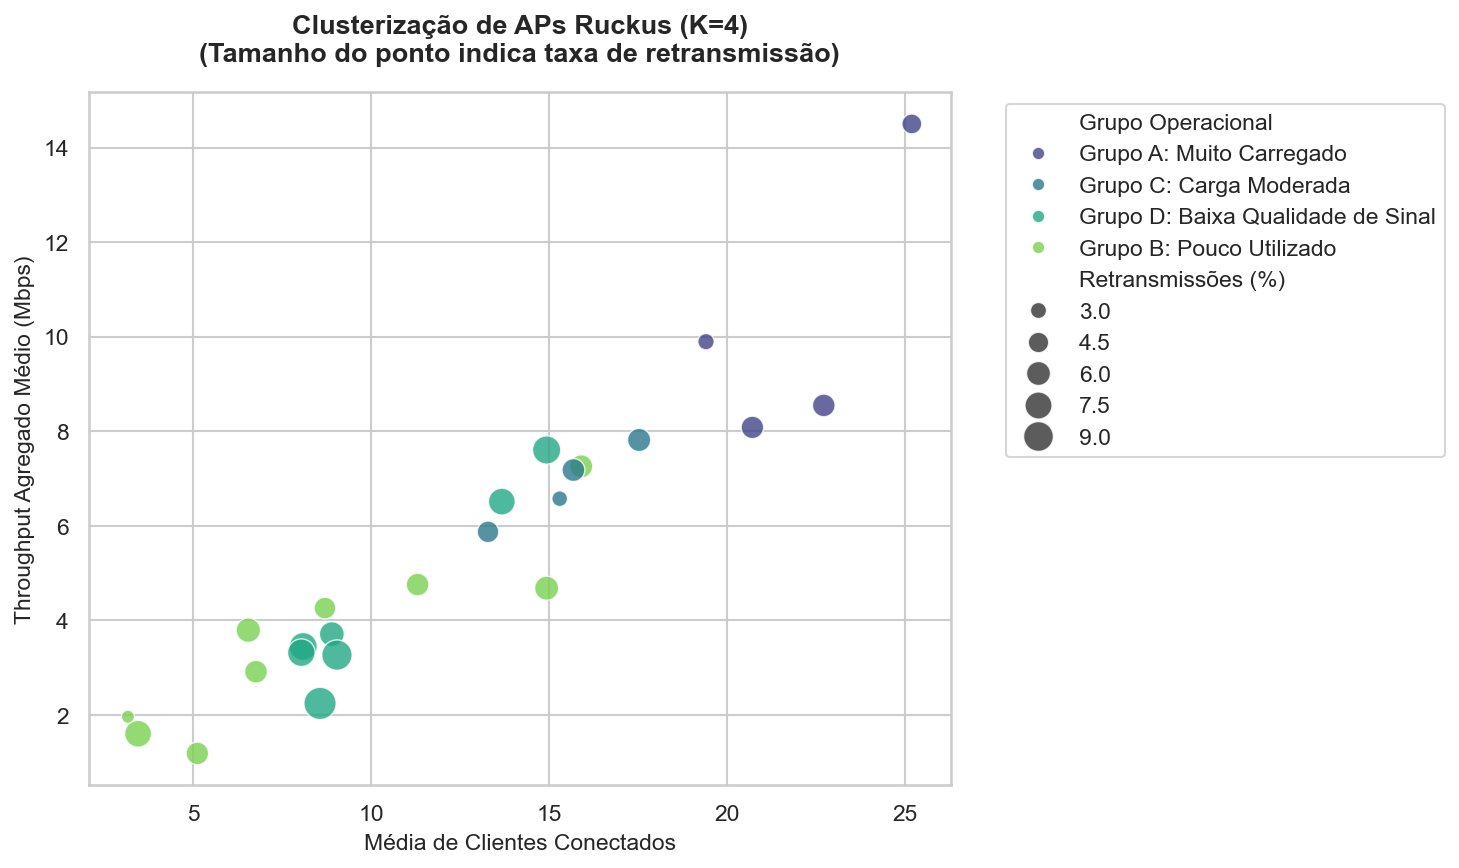
\includegraphics[width=0.85\textwidth]{img/cluster_ruckus.png}
  \caption{Clusterização Ruckus}
  \label{fig:cluster_ruckus_png}
\end{figure}

\begin{itemize}
  \item \textbf{UniFi}:
\end{itemize}
\begin{figure}[H]
  \centering
  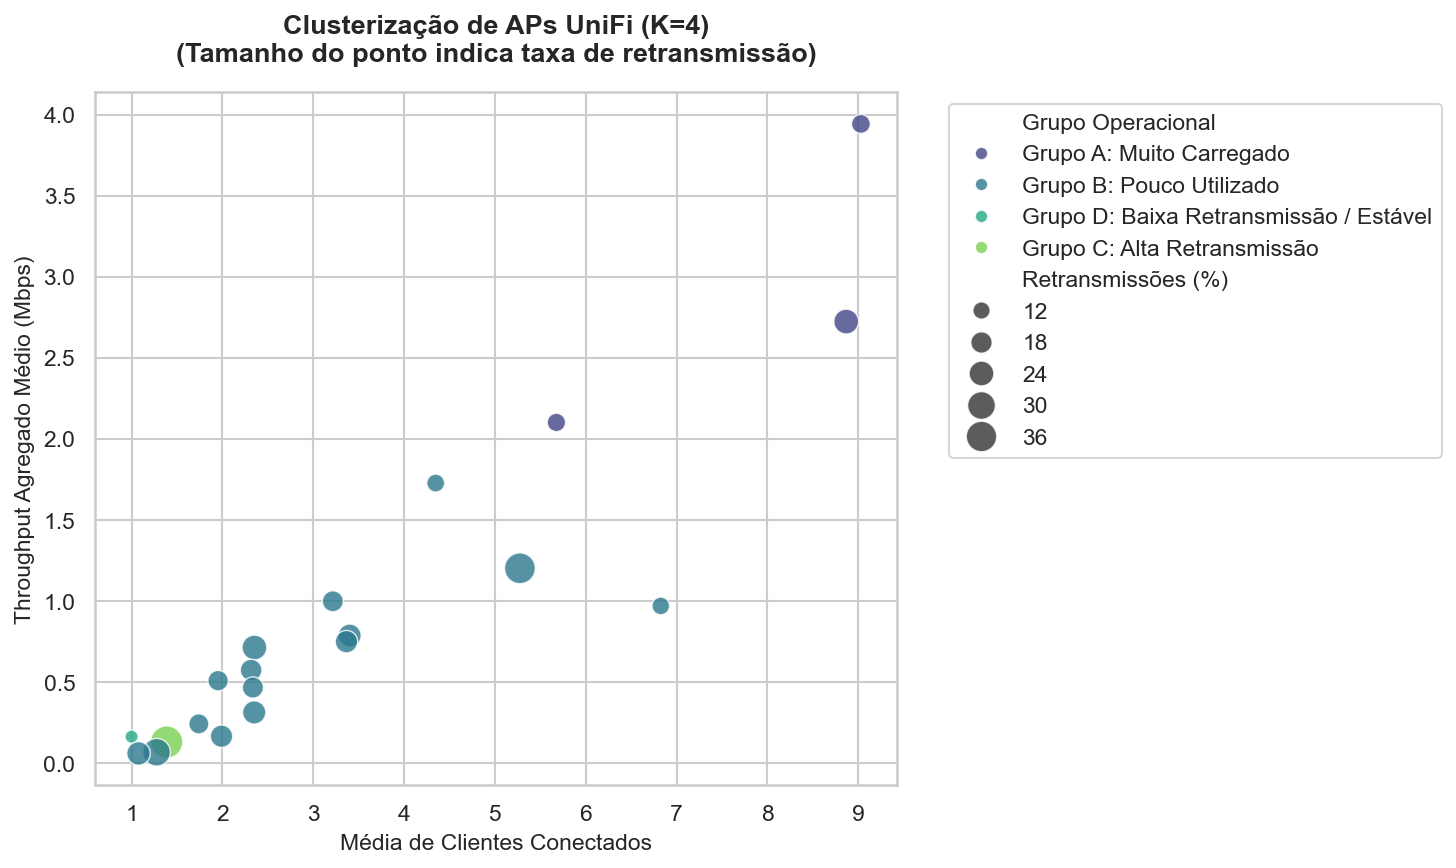
\includegraphics[width=0.85\textwidth]{img/cluster_unifi.png}
  \caption{Clusterização UniFi}
  \label{fig:cluster_unifi_png}
\end{figure}

